\chapter{Résolution du puzzle Link-Pix}

Le projet a connu différentes étapes de développement. En effet, le solveur étant lui-même découpé en plusieurs parties, nous avons tout d'abord travaillé sur la partie «~mise à jour~» des voisins, avant de passer à la construction des chemins. Nous avons ainsi une partie «~raffinage~» qui a pour objectif de simplifier le problème avant la résolution.

\section{De sous-problème en sous-problème}

\subsection{Modification des voisins}

La première partie du solveur vise à réduire l'ensemble des voisins possibles pour un indice. Ainsi, une coordonnée n'ayant qu'un voisin est, dans le cadre de puzzles qui ont une solution, le seul voisin possible de ce voisin-ci. On peut donc mettre à jour la liste des voisins de cette coordonnée.

Mais les anciens voisins peuvent également se retrouver à ce moment-là avec un unique voisin, il faut par conséquent répercuter la fonction sur eux si c'est le cas.

\begin{algorithm}
  \Data{$c_1$,$c_2$ des coordonnées, avec $c_1$ n'ayant que $c_2$ comme voisin \;
TabVoisin la structure contenant tous les voisins pour chaque coordonnée \;}
\Var{L1, une liste de coordonnées \;}
$L1 \gets TabVoisins\_getVoisins(c_2)$ \;
\ForEach{coordonnée $e$ \De L1}{
  \Si{$e \neq c_1 $}{
    $oterVoisin(c_2,e,TabVoisins)$ \;
    $supprimerdansLCoord(e,L1)$ \;
  }
  $TabVoisins\_setVoisins(c_2,L1)$ \;
}
\caption{affecterVoisin, qui modifie la liste des voisins de $c_2$, avec $c_2$ étant l'unique voisin de $c_1$}
\end{algorithm}

Cette fonction appelle pour chaque coordonnée voisine de $c_2$ la fonction \verb$oterVoisin$. Cette dernière modifie la liste des voisins de $e$ pour supprimer $c_2$, et appelle \verb$affecterVoisin$ si la liste des voisins à la fin est de longueur 1.

\begin{algorithm}
\Data{$c_1$,$c_2$ des coordonnées \;
TabVoisins la structure contenant tous les voisins pour chaque coordonnées \;}
\Var{L1, une liste de coordonnées \;}
$L1 \gets TabVoisins\_getVoisins(c_2) $ \;
$supprimerdansLCoord(c_1,L1)$ \;
$TabVoisins\_setVoisins(c_2,L1)$ \;
\Si{L1 est de longueur 1}{
$affecterVoisin(c_2,$ l'élément de L1 $,TabVoisins)$ \;
}
\caption{oterVoisin, qui supprime $c_1$ de la liste des voisins de $c_2$}
\end{algorithm}

Ainsi, lorsque l'on a une coordonnée $c$ ayant un unique voisin, un appel d'\verb$affecterVoisin$ sur $c$ et son unique voisin se répercutera sur les autres coordonnées «~en contact~» avec ce couple-là. On peut ainsi espérer isoler de la sorte des couples de coordonnées, simplifiant ainsi le problème.

Ces fonctions se situent dans le module «~Mise à jour des voisins~» (fichiers \verb$majVoisins.c$ et \verb$majVoisins.h$) du programme (voir \ref{graphes-dependance}).

\subsection{Existence d'un chemin}

Un deuxième algorithme nous permettant de réduire la liste des voisins possibles est l'algorithme qui teste pour deux coordonnées données, supposées voisines, s'il existe un chemin entre ces deux. Ainsi, si aucun chemin n'existe, on peut en déduire que ces deux coordonnées ne sont en réalité pas voisines.

\begin{algorithm}[H]
  \Data{$c_1$, $c_2$ des coordonnées \;
    $d$ la distance qui doit être parcourue entre $c_1$ et $c_2$ \;
    TabVoisins la matrice contenant les chemins et les indices \;
    L une liste de coordonnées contenant les cases déjà parcourues \;}
  \Result{Le booléen qui vaut Vrai s'il existe un chemin.}
  \Var{L1, une liste de coordonnées \;
    $b$, un booléen \;}
  \Si{$NON(c_1 \in L)$}{
    $L \gets creerListe(c_1,L)$ \;
    $L1 \gets $Liste des cases adjacentes de $c_1$ \;
    \eSi{$d = 2$}{
      \Renvoyer $c_2 \in L1$ \;
    }
        {
          \Tq{NON $b$ ET $L1 \neq NULL$ ET $L1->info$ n'est pas occupée}{
            $b \gets existeChemin(L1->info,c_2,d-1,TabVoisins,L)$ \;
          }  
          \Renvoyer b \;
        }
  }
  \caption{existeChemin, qui teste s'il existe un chemin entre $c_1$ et $c_2$}
\end{algorithm}

Cet algorithme s'appelle de façon récursive et teste tous les chemins possibles, sans repasser deux fois par la même case.

La condition d'arrêt de cet algorithme est dans le cas où on a un chemin à parcourir de longueur 2. Dans ce cas-là, on teste si les cases sont adjacentes. Si ce n'est pas le cas, on progresse comme indiqué dans la partie analyse, en se déplaçant sur les cases adjacentes et en testant s'il existe un chemin de longueur $d-1$.

On pourra ainsi réduire la liste des coordonnées voisines possibles grâce à cette fonction de «~tamisage~», avant de passer à la partie construction.

\subsection{Construction du début d'un chemin}

La construction d'un chemin, ou plus «~simplement~» du début d'un chemin, peut permettre d'éliminer de nouvelles possibilités pour les listes de voisins possibles.

Ainsi, un chemin, même incomplet, permet la progression de la résolution du problème. L'algorithme que nous avons écrit est un algorithme récursif, qui écrit un morceau de chemin et qui, s'il le peut, le complète au fur et à mesure. On a ainsi la fonction qui construira les chemins, mais aussi une fonction qui permettra de «~raffiner~» les listes de voisins.

\begin{algorithm}[H]
  \Data{$c_1$, $c_2$ des coordonnées qui sont uniques voisines l'une de l'autre \;
    $d$ la distance qui doit être parcourue entre $c_1$ et $c_2$ \;
    TabVoisins la matrice contenant les chemins et les indices \;}
  \Result{Un booléen valant Vrai si la construction du chemin a progressé, Faux sinon.}
  \Var{L1, une liste de coordonnées \;
    $s$, un entier \;
    $c$, une coordonnée \;}
  \eSi{$d = 2$}{
    Mettre à jour la grille avec 1 comme nouvelle valeur pour $c_1$ et $c_2$ \;
    \Renvoyer Vrai \;
  }
  {
    $s \gets 0$ \; 
    $L \gets$ Liste des cases adjacentes joignables \;
    \ForEach{coordonnées $e$ \De L}{
      \Si{existeChemin($e$,$c_2$,TabVoisins,NULL)}{$s \gets s+1$ \;
      $c \gets e$ \;}
    }

    \eSi{$s = 1$}{
      Mettre à jour la grille avec 1 pour $c_1$, et $d-1$ pour $c$ et $c_2$ \;
      $consChemin(c,c_2,d-1,TabVoisins)$ \;
      \Renvoyer Vrai \;
    }
        {
          \Renvoyer Faux \;
        }
  }
  \caption{consChemin, qui construit le début d'un chemin (si possible) entre $c_1$ et $c_2$}
\end{algorithm}

Cette fonction va s'arrêter si elle arrive dans le cas de deux indices adjacents et de chemin 2, ou dans le cas où il existe plus d'un début de chemin entre $c_1$ et $c_2$.
S'il n'existe qu'un seul début de chemin possible, elle va alors construire ce début de chemin. Elle va ensuite se positionner sur ce début de chemin, via l'appel récursif, et tenter à nouveau de construire un morceau de chemin.

On pourra aussi appeler cette fonction dans l'autre «~sens~». Car, en effet, il est possible que l'on ne puisse pas construire de morceau de chemin d'une coordonnée vers l'autre, mais que ce soit possible dans l'autre sens.

\section{Solveur}
  
Le solveur en lui-même est une succession d'appel sur les fonctions précédentes. On va ainsi «~tamiser~» le problème, tenter de voir si l'on a alors des chemins possibles, puis re-tamiser le problème, et ainsi de suite jusqu'à ce que la solution apparaisse. La structure globale du solveur sera alors :

\begin{algorithm}[H]
  \Tq{le problème n'est pas résolu}{
    Tamiser le problème \;
    Construire des morceaux de chemins \;
  }
  \caption{Structure globale du solveur}
\end{algorithm}

La boucle principale se décomposera ainsi en deux sous-parties, appelant chacune des fonctions décrites dans la section précédente.

\subsection{Boucle principale}

Pour représenter le fait que le problème n'est pas encore résolu, nous avons fait le choix d'utiliser deux listes.

\begin{figure}[h]
      \centering
      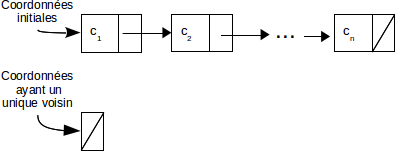
\includegraphics[scale=0.5]{solveur-listes}
      \caption{Valeur des listes au début de la résolution}
\end{figure}

La première liste contient toutes les coordonnées de la grille qui n'ont pas été traitées, tandis que la seconde liste contient les coordonnées qui auront été analysées par le «~tamisage~» mais dont on n'aura pas encore construit le chemin. Ainsi, après le tamisage, les listes seraient de la forme :

\begin{figure}[h]
      \centering
      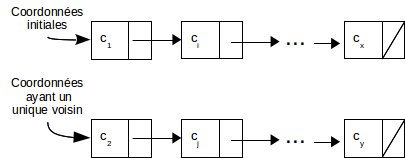
\includegraphics[scale=0.5]{solveur-listes2}
      \caption{Valeur des listes après tamisage}
\end{figure}

La partie construction, quant à elle, ne toucherait pas pas à la liste des coordonnées initiales mais modifierait la liste des coordonnées ayant un unique voisin, supprimant celles qui ont leurs chemins complétés.


\begin{figure}[h!]
      \centering
      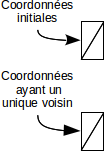
\includegraphics[scale=0.5]{solveur-listes3}
      \caption{Valeur des listes à la fin de la résolution}
\end{figure}

La résolution serait alors finie quand les deux listes seraient vides.

\subsection{Tamisage}

La partie tamisage du solveur serait principalement composé des fonctions de mise à jour des voisins dans le cas de coordonnées ayant un voisin unique ainsi que de la fonction qui teste s'il existe un chemin entre deux coordonnées.

La première partie du tamisage serait alors d'essayer, pour chaque coordonnées n'ayant qu'un unique voisin, de faire se répercuter ceci sur les autres coordonnées. 

\begin{algorithm}[H]
  \ForEach{coordonnées c \De la liste initiale}{
    \Si{$c$ n'a qu'un seul voisin}{
      $affecterVoisin(c,voisin de c,TabVoisins)$ \;
    }
  }
  \caption{Première partie du tamisage}
\end{algorithm}

La fonction \verb$affecterVoisin$ devrait ainsi également modifier la liste initiale, retirant les éléments modifiés et n'ayant plus qu'un unique voisin.

La seconde partie du tamisage consisterait, pour chaque couple de coordonnées supposées voisines, à tester si un chemin existe entre elles. Si ce n'est pas le cas, alors, on doit supprimer le lien de «~voisinage~» qui existe entre elles.

\begin{algorithm}[H]
  \ForEach{coordonnée $c$ \De la liste initiale}{
    \ForEach{coordonnée $c_2$ \De la liste des voisins de $c$}{
      \Si{NON($existeChemin(c,c_2,valeur de c,TabVoisins,NULL)$}{
        Retirer $c$ de la liste des voisins de $c_2$ \;
        Retirer $c_2$ de la liste des voisins de $c$ \;
      }
    }
  }
  \caption{Deuxième partie du tamisage}
\end{algorithm}

On pourra également après appeler affecterVoisin sur ces coordonnées dans le cas où, après retrait, il n'existerait plus qu'un seul voisin possible.

\subsection{Construction}

Dans cette partie, le solveur tenterait de créer des chemins ou, si un chemin complet n'est pas possible, des morceaux de chemins dans le but d'affiner le problème lors du tamisage suivant.

\begin{algorithm}[H]
  \ForEach{coordonnées $c$ \De la liste des coordonnées ayant un unique voisin}{
    consChemin($c$,voisin de $c$,valeur de $c$,TabVoisins) \;
  }
  \caption{Construction des chemins}
\end{algorithm}

La fonction \verb$consChemin$ devrait alors également modifier une liste du solveur. En effet, celle-ci devrait supprimer les coordonnées dont on a fini le chemin de la liste, ne laissant dedans que celles en attente de pouvoir progresser dans la construction du chemin.
